\scanpage{15}\mspage{14}
En résumé, en termes de $\unsure{\mathcal{F}|\mathfrak{F}}$, c'est de la donnée de deux \uline{relations} \uline{d'ordre}
% The enclosure has separate top, left and bottom strokes; no right vertical is visible.
\figure{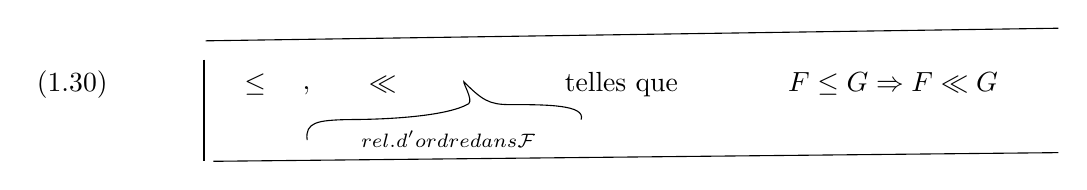
\begin{tikzpicture}[x=1cm,y=1cm]
  \node[anchor=east] at (-1.1,0.68) {$(1.30)$};
  \node at (0.65,0.68) {$\leq$};
  \node at (1.30,0.59) {$,$};
  \node at (2.27,0.68) {$\ll$};
  \node at (5.30,0.68) {telles que};
  \node at (8.75,0.68) {$F\leq G\Rightarrow F\ll G$};
  \node at (3.10,-0.02) {$\scriptstyle\text{rel. d'ordre dans }\mathcal{F}$};
  \draw (0.02,1.23) -- (10.85,1.39);
  \draw (0,0.99) -- (0,-0.30);
  \draw (0.12,-0.30) -- (10.85,-0.19);
  \draw (1.31,-0.03) .. controls (1.28,0.20) and (1.45,0.22) .. (1.82,0.23)
    .. controls (2.40,0.23) and (3.10,0.28) .. (3.36,0.43)
    .. controls (3.42,0.48) and (3.29,0.69) .. (3.30,0.71)
    .. controls (3.53,0.48) and (3.62,0.42) .. (3.88,0.42)
    .. controls (4.34,0.42) and (4.85,0.42) .. (4.79,0.23);
\end{tikzpicture}}
que je vais partir.

En termes de celles-ci, on definit \deleted{$\unsure{\mathcal{M}|M}$}
\[
\mathcal{M}\subset\mathcal{F}
\]
par (1.20), avec les relations $\underset{\mathcal{M}}{\leq},\ \underset{\mathcal{M}}{\ll}$ induites par $\underset{\mathcal{F}}{\leq},\ \underset{\unsure{\mathcal{F}|\overline{f}}}{\ll}$, puis
\[
\mathcal{L}\subset\mathcal{M}
\]
par (1.25). L'application
\[
\mathcal{F}\hookrightarrow\unsure{\mathcal{P}|\mathscr{P}|\mathfrak{P}}(\mathcal{M})\qquad
\mathord{\rlap{$\deleted{X}$}F}\longmapsto\widetilde F=\mathrm{Dep}(F)
\tag*{($*$)}
\]
% The input X is overwritten by F at the same horizontal position.
est \inserted{alors} definie par
\[
\widetilde F=\{X\in\mathcal{M}\mid X\leq F\}
\tag*{(1.31)}
\]
et
\[
\mathcal{F}\hookrightarrow\mathrm{Fig}(\mathcal{M})\qquad
\unsure{F|\deleted{X}F}\longmapsto\mathrm{Fig}_{\mathcal{M}}(F)
\tag*{($**$)}
\]
% At the second map an extra diagonal crosses F; a canceled X is possible, not established.
par (1.4) :
\[
\mathrm{Fig}_{\mathcal{M}}(F)=\{\widetilde X\mid X\in\widetilde F\}\subset\mathcal{P}(\mathcal{M})
\tag*{\deleted{(1.32)}}
\]
avec
\[
\widetilde X=\{Y\in\mathcal{M}\mid Y\leq X\}\quad.
\]

Ainsi, $\mathcal{F}$ est interprété comme un ens. de parties dans $\mathcal{M}$ via ($*$), et $\leq$ \unsure{s'interprète|s'interprête} simplement par l'inclusion
\[
F\leq G\Longleftrightarrow\widetilde F\subset\widetilde G
\tag*{(1.32)}
\]
